% answers.tex —— 2008 年·普通高等学校招生考试·辽宁卷·文科 · 参考答案与详细解析片段
% 由 tools/generate_projects.py 依来源总账自 2008/2008_数学真题_辽宁文_试题.md + 2008/2008_数学真题_辽宁文_解析正文.md + 2008/2008_数学真题_辽宁文_答案要点.md 生成，勿手改（改源 MD 后重跑）


\begin{gktip}
固定候选 PDF 仅含题面，无答案、解析和评分标准，原卷亦未标注分值；以下为非官方编者独立推导，官方答案字段为空。来源发布者、出版者、版次与官方身份均未核。
\end{gktip}

\begin{answer}
\gksolhead{1}{}

\textbf{题目}：

已知集合 $M=\{x\mid -3<x<1\}$，$N=\{x\mid x\leqslant-3\}$，则 $M\cup N=$（　）

（A）$\varnothing$

（B）$\{x\mid x\geqslant-3\}$

（C）$\{x\mid x\geqslant1\}$

（D）$\{x\mid x<1\}$

\Needspace{4\baselineskip}
\textbf{解析}

\Needspace{5\baselineskip}
$M=(-3,1)$，$N=(-\infty,-3]$，故

\nopagebreak[4]
\[M\cup N=(-\infty,1)=\{x\mid x<1\}.\]

\gkanswer{答案：D。}

\end{answer}
\begin{answer}
\gksolhead{2}{}

\textbf{题目}：

若函数 $y=(x+1)(x-a)$ 为偶函数，则 $a=$（　）

（A）$-2$

（B）$-1$

（C）$1$

（D）$2$

\Needspace{4\baselineskip}
\textbf{解析}

$y=(x+1)(x-a)=x^2+(1-a)x-a$ 为偶函数，一次项系数为零，故 $a=1$。

\gkanswer{答案：C。}

\end{answer}
\begin{answer}
\gksolhead{3}{}

\textbf{题目}：

圆 $x^2+y^2=1$ 与直线 $y=kx+2$ 没有公共点的充要条件是（　）

（A）$k\in(-\sqrt2,\sqrt2)$

（B）$k\in(-\sqrt3,\sqrt3)$

（C）$k\in(-\infty,-\sqrt2)\cup(\sqrt2,+\infty)$

（D）$k\in(-\infty,-\sqrt3)\cup(\sqrt3,+\infty)$

\Needspace{4\baselineskip}
\textbf{解析}

\Needspace{5\baselineskip}
圆心到直线 $kx-y+2=0$ 的距离为 $\dfrac2{\sqrt{k^2+1}}$，无公共点等价于

\nopagebreak[4]
\[\frac2{\sqrt{k^2+1}}>1\iff k^2<3.\]

\gkanswer{答案：B。}

\end{answer}
\begin{answer}
\gksolhead{4}{}

\textbf{题目}：

已知 $0<a<1$，$x=\log_a\sqrt2+\log_a\sqrt3$，$y=\dfrac12\log_a5$，$z=\log_a\sqrt{21}-\log_a\sqrt3$，则（　）

（A）$x>y>z$

（B）$z>y>x$

（C）$y>x>z$

（D）$z>x>y$

\Needspace{4\baselineskip}
\textbf{解析}

$x=\log_a\sqrt6$，$y=\log_a\sqrt5$，$z=\log_a\sqrt{21}-\log_a\sqrt3=\log_a\sqrt7$。由 $0<a<1$ 知 $y=\log_a t$ 递减，而 $\sqrt5<\sqrt6<\sqrt7$，故 $y>x>z$。

\gkanswer{答案：C。}

\end{answer}
\begin{answer}
\gksolhead{5}{}

\textbf{题目}：

已知四边形 $ABCD$ 的三个顶点 $A(0,2)$，$B(-1,-2)$，$C(3,1)$，且 $\overrightarrow{BC}=2\overrightarrow{AD}$，则顶点 $D$ 的坐标为（　）

（A）$\left(2,\dfrac72\right)$

（B）$\left(2,-\dfrac12\right)$

（C）$(3,2)$

（D）$(1,3)$

\Needspace{4\baselineskip}
\textbf{解析}

\Needspace{5\baselineskip}
$\overrightarrow{BC}=(4,3)$，由 $\overrightarrow{BC}=2\overrightarrow{AD}$ 得 $\overrightarrow{AD}=(2,\tfrac32)$，故

\nopagebreak[4]
\[D=A+\overrightarrow{AD}=\left(2,\frac72\right).\]

\gkanswer{答案：A。}

\end{answer}
\begin{answer}
\gksolhead{6}{}

\textbf{题目}：

设 $P$ 为曲线 $C:y=x^2+2x+3$ 上的点，且曲线 $C$ 在点 $P$ 处切线倾斜角的取值范围是 $\left[0,\dfrac{\pi}{4}\right]$，则点 $P$ 横坐标的取值范围是（　）

（A）$\left[-1,-\dfrac12\right]$

（B）$[-1,0]$

（C）$[0,1]$

（D）$\left[\dfrac12,1\right]$

\Needspace{4\baselineskip}
\textbf{解析}

\Needspace{5\baselineskip}
$y'=2x+2$。切线倾斜角 $\theta\in[0,\tfrac{\pi}{4}]$ 即 $\tan\theta\in[0,1]$，故

\nopagebreak[4]
\[0\leqslant 2x+2\leqslant 1\iff -1\leqslant x\leqslant-\frac12.\]

\gkanswer{答案：A。}

\end{answer}
\begin{answer}
\gksolhead{7}{}

\textbf{题目}：

$4$ 张卡片上分别写有数字 $1$，$2$，$3$，$4$，从这 $4$ 张卡片中随机抽取 $2$ 张，则取出的 $2$ 张卡片上的数字之和为奇数的概率为（　）

（A）$\dfrac13$

（B）$\dfrac12$

（C）$\dfrac23$

（D）$\dfrac34$

\Needspace{4\baselineskip}
\textbf{解析}

和为奇数需一奇一偶，取法 $2\times2=4$ 种，总取法 $\mathrm C_4^2=6$，故概率为 $\dfrac23$。

\gkanswer{答案：C。}

\end{answer}
\begin{answer}
\gksolhead{8}{}

\textbf{题目}：

将函数 $y=2^x+1$ 的图象按向量 $\boldsymbol a$ 平移得到函数 $y=2^{x+1}$ 的图象，则（　）

（A）$\boldsymbol a=(-1,-1)$

（B）$\boldsymbol a=(1,-1)$

（C）$\boldsymbol a=(1,1)$

（D）$\boldsymbol a=(-1,1)$

\Needspace{4\baselineskip}
\textbf{解析}

设平移向量 $\boldsymbol a=(h,k)$，则新图象为 $y=2^{x-h}+1+k$，与 $y=2^{x+1}$ 比较得 $h=-1$，$k=-1$。

\gkanswer{答案：A。}

\end{answer}
\begin{answer}
\gksolhead{9}{}

\textbf{题目}：

已知变量 $x$，$y$ 满足约束条件 $\begin{cases}y+x-1\leqslant0,\\ y-3x-1\leqslant0,\\ y-x+1\geqslant0,\end{cases}$ 则 $z=2x+y$ 的最大值为（　）

（A）$4$

（B）$2$

（C）$1$

（D）$-4$

\Needspace{4\baselineskip}
\textbf{解析}

三直线两两相交得可行域顶点：$x+y=1$ 与 $y=x-1$ 交于 $(1,0)$；$x+y=1$ 与 $y=3x+1$ 交于 $(0,1)$；$y=x-1$ 与 $y=3x+1$ 交于 $(-1,-2)$。对应 $z=2x+y$ 为 $2$、$1$、$-4$，最大值为 $2$。

\gkanswer{答案：B。}

\end{answer}
\begin{answer}
\gksolhead{10}{}

\textbf{题目}：

一生产过程有 $4$ 道工序，每道工序需要安排一人照看。现从甲、乙、丙等 $6$ 名工人中安排 $4$ 人分别照看一道工序，第一道工序只能从甲、乙两工人中安排 $1$ 人，第四道工序只能从甲、丙两工人中安排 $1$ 人，则不同的安排方案共有（　）

（A）$24$ 种

（B）$36$ 种

（C）$48$ 种

（D）$72$ 种

\Needspace{4\baselineskip}
\textbf{解析}

第一道由甲承担：第四道只能由丙承担，余下两道从余下 $4$ 人中选排 $\mathrm A_4^2=12$ 种。

第一道由乙承担：第四道可由甲或丙承担（$2$ 种），余下两道 $\mathrm A_4^2=12$ 种，共 $24$ 种。

合计 $12+24=36$ 种。

\gkanswer{答案：B。}

\end{answer}
\begin{answer}
\gksolhead{11}{}

\textbf{题目}：

已知双曲线 $9y^2-m^2x^2=1$（$m>0$）的一个顶点到它的一条渐近线的距离为 $\dfrac15$，则 $m=$（　）

（A）$1$

（B）$2$

（C）$3$

（D）$4$

\Needspace{4\baselineskip}
\textbf{解析}

\Needspace{5\baselineskip}
双曲线即 $\dfrac{y^2}{1/9}-\dfrac{x^2}{1/m^2}=1$，顶点为 $\left(0,\pm\tfrac13\right)$，渐近线 $mx-3y=0$。由

\nopagebreak[4]
\[\frac{\left|m\cdot0-3\cdot\frac13\right|}{\sqrt{m^2+9}}=\frac15\iff\sqrt{m^2+9}=5\]

得 $m=4$。

\gkanswer{答案：D。}

\end{answer}
\begin{answer}
\gksolhead{12}{}

\textbf{题目}：

在正方体 $ABCD-A_1B_1C_1D_1$ 中，$E$，$F$ 分别为棱 $AA_1$，$CC_1$ 的中点，则在空间中与三条直线 $A_1D_1$，$EF$，$CD$ 都相交的直线（　）

（A）不存在

（B）有且只有两条

（C）有且只有三条

（D）有无数条

\Needspace{4\baselineskip}
\textbf{解析}

取 $A(0,0,0)$、$B(1,0,0)$、$C(1,1,0)$、$D(0,1,0)$，则 $E\left(0,0,\tfrac12\right)$、$F\left(1,1,\tfrac12\right)$；$A_1D_1$ 为 $\{(0,t,1)\}$，$EF$ 为 $\{(u,u,\tfrac12)\}$，$CD$ 为 $\{(s,1,0)\}$。

对每个 $u\in[0,1]$，点 $(u,u,\tfrac12)$ 可与 $A_1D_1$ 上一点、$CD$ 上一点共线，得到一条与三条直线都相交的直线；$u$ 连续变化给出无穷多条互不相同的直线，故有无数条。

\gkanswer{答案：D。}

\end{answer}
\begin{answer}
\gksolhead{13}{}

\textbf{题目}：

函数 $y=\mathrm e^{2x+1}$（$-\infty<x<+\infty$）的反函数是\gkblank{}。

\Needspace{4\baselineskip}
\textbf{解析}

\Needspace{5\baselineskip}
由 $y=\mathrm e^{2x+1}$ 得 $2x+1=\ln y$，即 $x=\dfrac{\ln y-1}{2}$。交换 $x$、$y$ 得反函数

\nopagebreak[4]
\[y=\frac12(\ln x-1)\quad(x>0).\]

\gkanswer{答案：$y=\dfrac12(\ln x-1)$（$x>0$）。}

\end{answer}
\begin{answer}
\gksolhead{14}{}

\textbf{题目}：

在体积为 $4\sqrt3\pi$ 的球的表面上有 $A$，$B$，$C$ 三点，$AB=1$，$BC=\sqrt2$，$A$，$C$ 两点的球面距离为 $\dfrac{\sqrt3}{3}\pi$，则球心到平面 $ABC$ 的距离为\gkblank{}。

\Needspace{4\baselineskip}
\textbf{解析}

\Needspace{5\baselineskip}
由 $\dfrac43\pi R^3=4\sqrt3\pi$ 得 $R=\sqrt3$。球面距离 $\dfrac{\sqrt3}{3}\pi=R\theta$ 给 $\theta=\dfrac{\pi}{3}$，故

\nopagebreak[4]
\[AC=2R\sin\frac{\theta}{2}=\sqrt3.\]

\Needspace{5\baselineskip}
于是 $AB^2+BC^2=1+2=3=AC^2$，$\triangle ABC$ 为直角三角形，外接圆半径 $r=\dfrac{AC}{2}=\dfrac{\sqrt3}{2}$。球心到平面的距离为

\nopagebreak[4]
\[\sqrt{R^2-r^2}=\sqrt{3-\frac34}=\frac32.\]

\gkanswer{答案：$\dfrac32$。}

\end{answer}
\begin{answer}
\gksolhead{15}{}

\textbf{题目}：

$\left(1+x^3\right)\left(x+\dfrac1{x^2}\right)^6$ 展开式中的常数项为\gkblank{}。

\Needspace{4\baselineskip}
\textbf{解析}

$\left(x+\dfrac1{x^2}\right)^6$ 的通项为 $\mathrm C_6^kx^{6-k}\cdot x^{-2k}=\mathrm C_6^kx^{6-3k}$。

乘 $1$ 时取 $k=2$，常数项 $\mathrm C_6^2=15$；乘 $x^3$ 时需 $6-3k+3=0$，即 $k=3$，常数项 $\mathrm C_6^3=20$。

故常数项为 $15+20=35$。

\gkanswer{答案：$35$。}

\end{answer}
\begin{answer}
\gksolhead{16}{}

\textbf{题目}：

设 $x\in\left(0,\dfrac{\pi}{2}\right)$，则函数 $y=\dfrac{2\sin^2x+1}{\sin2x}$ 的最小值为\gkblank{}。

\Needspace{4\baselineskip}
\textbf{解析}

\nopagebreak[4]
\[y=\frac{2\sin^2x+\sin^2x+\cos^2x}{2\sin x\cos x}=\frac{3\sin^2x+\cos^2x}{2\sin x\cos x}=\frac{3\tan^2x+1}{2\tan x}.\]

\Needspace{5\baselineskip}
令 $t=\tan x>0$，则

\nopagebreak[4]
\[y=\frac12\left(3t+\frac1t\right)\geqslant\frac12\cdot2\sqrt3=\sqrt3,\]

当 $3t=\dfrac1t$ 即 $t=\dfrac1{\sqrt3}$（$x=\dfrac{\pi}{6}$）时取等号，故最小值为 $\sqrt3$。

\gkanswer{答案：$\sqrt3$。}

\end{answer}
\begin{answer}
\gksolhead{17}{}

\textbf{题目}：

在 $\triangle ABC$ 中，内角 $A$，$B$，$C$ 对边的边长分别是 $a$，$b$，$c$。已知 $c=2$，$C=\dfrac{\pi}{3}$。

（1）若 $\triangle ABC$ 的面积等于 $\sqrt3$，求 $a$，$b$；

（2）若 $\sin B=2\sin A$，求 $\triangle ABC$ 的面积。

\Needspace{4\baselineskip}
\textbf{解析}

（1）$S=\dfrac12ab\sin C=\dfrac{\sqrt3}{4}ab=\sqrt3$，故 $ab=4$。

由余弦定理 $c^2=a^2+b^2-2ab\cos C$ 得 $a^2+b^2-ab=4$，即 $a^2+b^2=8$。于是 $(a+b)^2=8+8=16$，$a+b=4$，结合 $ab=4$ 得 $a=b=2$。

\Needspace{5\baselineskip}
（2）由正弦定理，$\sin B=2\sin A$ 等价于 $b=2a$。代入 $a^2+b^2-ab=4$ 得 $3a^2=4$，$a^2=\dfrac43$。故

\nopagebreak[4]
\[S=\frac12ab\sin C=\frac12\cdot2a^2\cdot\frac{\sqrt3}{2}=\frac{2\sqrt3}{3}.\]

\gkanswer{答案：（1）$a=b=2$；（2）$\dfrac{2\sqrt3}3$。}

\end{answer}
\begin{answer}
\gksolhead{18}{}

\textbf{题目}：

某批发市场对某种商品的周销售量（单位：吨）进行统计，最近 $100$ 周的统计结果如下表所示：

\begin{center}
\begin{tabular}{llll}
\toprule
周销售量 & $2$ & $3$ & $4$ \\
\midrule
频数 & $20$ & $50$ & $30$ \\
\bottomrule
\end{tabular}
\end{center}

（1）根据上面统计结果，求周销售量分别为 $2$ 吨、$3$ 吨和 $4$ 吨的频率；

（2）若以上述频率作为概率，且各周的销售量相互独立，求

① $4$ 周中该种商品至少有一周的销售量为 $4$ 吨的概率；

② 该种商品 $4$ 周的销售量总和至少为 $15$ 吨的概率。

\Needspace{4\baselineskip}
\textbf{解析}

\Needspace{5\baselineskip}
（1）频率依次为

\nopagebreak[4]
\[\frac{20}{100}=0.2,\qquad\frac{50}{100}=0.5,\qquad\frac{30}{100}=0.3.\]

\Needspace{5\baselineskip}
（2）① 四周都不到 $4$ 吨的概率为 $0.7^4=0.2401$，故至少一周为 $4$ 吨的概率为

\nopagebreak[4]
\[1-0.2401=0.7599.\]

\Needspace{5\baselineskip}
② 四周总量至少 $15$ 吨只有两种情形：四周均为 $4$ 吨，或三周为 $4$ 吨、一周为 $3$ 吨。故

\nopagebreak[4]
\[P=0.3^4+\mathrm C_4^1\cdot0.3^3\cdot0.5=0.0081+0.054=0.0621.\]

\gkanswer{答案：（1）$0.2$，$0.5$，$0.3$；（2）① $0.7599$；② $0.0621$。}

\end{answer}
\begin{answer}
\gksolhead{19}{}

\textbf{题目}：

如图，在棱长为 $1$ 的正方体 $ABCD-A'B'C'D'$ 中，$AP=BQ=b$（$0<b<1$），截面 $PQEF\parallel A'D$，截面 $PQGH\parallel AD'$。

（1）证明：平面 $PQEF$ 和平面 $PQGH$ 互相垂直；

（2）证明：截面 $PQEF$ 和截面 $PQGH$ 面积之和是定值，并求出这个值；

（3）若 $b=\dfrac12$，求 $D'E$ 与平面 $PQEF$ 所成角的正弦值。
\nopagebreak[4]
\begin{center}% 2008 年辽宁卷文科第 19 题：棱长 1 的正方体 ABCD-A'B'C'D'，AP=BQ=b，
%   截面 PQEF∥A'D，截面 PQGH∥AD'。
% 来源 PDF：gaokaomath-src/普通高考/2008/2008辽宁文.pdf
% SHA-256：9f2a8aeabda218eb3460fd8035aaf894f32be8ff5b0a3427d379552bd0233a65
% 原页：2008辽宁文.pdf 第 56 页? 按印面页码 465–466，本图在第 1 页第 3 栏。
% 重绘依据：按原页斜投影取 A 前左下、B 前右下、C 右后下、D 被遮挡；A'B'C'D' 为顶面；
%   P 在 AA' 上、Q 在 BB' 上、E 在 BC 上、F 在 AD 上、G 在 B'C' 上、H 在 A'D' 上，
%   两侧截面以实线闭合，隐藏棱与 A'D、AD' 两条对角线用虚线。
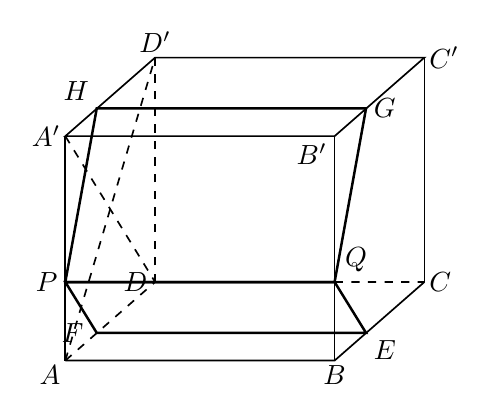
\begin{tikzpicture}[scale=0.95, semithick, every node/.style={inner sep=1.5pt}]
  \coordinate (A) at (0.00,0.00);
  \coordinate (B) at (3.60,0.00);
  \coordinate (C) at (4.80,1.05);
  \coordinate (D) at (1.20,1.05);
  \coordinate (A1) at (0.00,3.00);
  \coordinate (B1) at (3.60,3.00);
  \coordinate (C1) at (4.80,4.05);
  \coordinate (D1) at (1.20,4.05);

  \coordinate (P) at (0.00,1.05);
  \coordinate (Q) at (3.60,1.05);
  \coordinate (E) at (4.02,0.37);
  \coordinate (F) at (0.42,0.37);
  \coordinate (G) at (4.02,3.37);
  \coordinate (H) at (0.42,3.37);

  % 立方体可见棱
  \draw (A) -- (B) -- (C);
  \draw (A) -- (A1);
  \draw (B) -- (B1);
  \draw (C) -- (C1);
  \draw (A1) -- (B1) -- (C1) -- (D1) -- cycle;

  % 隐藏棱
  \draw[dashed] (A) -- (D) -- (C);
  \draw[dashed] (D) -- (D1);

  % 两个截面
  \draw[line width=0.9pt] (P) -- (Q) -- (E) -- (F) -- cycle;
  \draw[line width=0.9pt] (P) -- (Q) -- (G) -- (H) -- cycle;

  % 与截面平行的两条对角线
  \draw[dashed] (A1) -- (D);
  \draw[dashed] (A) -- (D1);

  \node[below left] at (A) {$A$};
  \node[below] at (B) {$B$};
  \node[right] at (C) {$C$};
  \node[left=1pt] at (D) {$D$};
  \node[left] at (A1) {$A'$};
  \node[below left=1pt] at (B1) {$B'$};
  \node[right] at (C1) {$C'$};
  \node[above] at (D1) {$D'$};
  \node[left=1pt] at (P) {$P$};
  \node[above right=2pt] at (Q) {$Q$};
  \node[below right=1pt] at (E) {$E$};
  \node[left=3pt] at (F) {$F$};
  \node[right=1pt] at (G) {$G$};
  \node[above left=1pt] at (H) {$H$};
\end{tikzpicture}
\end{center}
\nopagebreak[4]
\Needspace{4\baselineskip}
\textbf{解析}

\Needspace{5\baselineskip}
以 $A$ 为原点，$AB$、$AD$、$AA'$ 为 $x$、$y$、$z$ 轴，棱长为 $1$，则

\nopagebreak[4]
\[P(0,0,b),\quad Q(1,0,b),\quad E(1,b,0),\quad F(0,b,0),\quad G(1,1-b,1),\quad H(0,1-b,1).\]

\Needspace{5\baselineskip}
（1）平面 $PQEF$ 含 $\overrightarrow{PQ}=(1,0,0)$ 与 $\overrightarrow{A'D}=(0,1,-1)$，法向量

\nopagebreak[4]
\[\boldsymbol n_1=\overrightarrow{PQ}\times\overrightarrow{A'D}=(0,1,1).\]

\Needspace{5\baselineskip}
平面 $PQGH$ 含 $\overrightarrow{PQ}$ 与 $\overrightarrow{AD'}=(0,1,1)$，法向量

\nopagebreak[4]
\[\boldsymbol n_2=\overrightarrow{PQ}\times\overrightarrow{AD'}=(0,-1,1).\]

由 $\boldsymbol n_1\cdot\boldsymbol n_2=-1+1=0$ 知两平面互相垂直。

\Needspace{5\baselineskip}
（2）$PQEF$ 为矩形，$PQ=1$，$QE=\left|(0,b,-b)\right|=b\sqrt2$，面积 $S_1=\sqrt2b$；同理 $PQGH$ 为矩形，$PG=\left|(0,1-b,1-b)\right|=(1-b)\sqrt2$，面积 $S_2=\sqrt2(1-b)$。故

\nopagebreak[4]
\[S_1+S_2=\sqrt2\]

为定值。

\Needspace{5\baselineskip}
（3）$b=\dfrac12$ 时 $\boldsymbol n_1=(0,1,1)$，$\overrightarrow{D'E}=\left(1,-\dfrac12,-1\right)$，故

\nopagebreak[4]
\[\sin\theta=\frac{\left|\overrightarrow{D'E}\cdot\boldsymbol n_1\right|}{\left|\overrightarrow{D'E}\right|\left|\boldsymbol n_1\right|}=\frac{\left|-\frac12-1\right|}{\frac32\cdot\sqrt2}=\frac{\sqrt2}{2}.\]

\gkanswer{答案：（1）证明见解析；（2）定值 $\sqrt2$；（3）$\dfrac{\sqrt2}2$。}

\end{answer}
\begin{answer}
\gksolhead{20}{}

\textbf{题目}：

在数列 $\{a_n\}$，$\{b_n\}$ 是各项均为正数的等比数列，设 $c_n=\dfrac{b_n}{a_n}$（$n\in\mathbf N^*$）。

（1）数列 $\{c_n\}$ 是否为等比数列？证明你的结论；

（2）设数列 $\{\ln a_n\}$，$\{\ln b_n\}$ 的前 $n$ 项和分别为 $S_n$，$T_n$。若 $a_1=2$，$\dfrac{S_n}{T_n}=\dfrac{n}{2n+1}$，求数列 $\{c_n\}$ 的前 $n$ 项和。

\Needspace{4\baselineskip}
\textbf{解析}

\Needspace{5\baselineskip}
（1）设 $\{a_n\}$、$\{b_n\}$ 的公比分别为 $q_1$、$q_2$，则

\nopagebreak[4]
\[\frac{c_{n+1}}{c_n}=\frac{b_{n+1}}{b_n}\cdot\frac{a_n}{a_{n+1}}=\frac{q_2}{q_1}\]

为与 $n$ 无关的常数，故 $\{c_n\}$ 是等比数列。

\Needspace{5\baselineskip}
（2）记 $u=\ln a_1$，$v=\dfrac12\ln q_1$，$U=\ln b_1$，$V=\dfrac12\ln q_2$，则

\nopagebreak[4]
\[S_n=nu+n(n-1)v,\qquad T_n=nU+n(n-1)V.\]

\Needspace{5\baselineskip}
由 $\dfrac{S_n}{T_n}=\dfrac{n}{2n+1}$ 得

\nopagebreak[4]
\[(2n+1)\bigl(u+(n-1)v\bigr)=nU+n(n-1)V.\]

\Needspace{5\baselineskip}
比较 $n^2$ 项、$n$ 项与常数项系数，得

\nopagebreak[4]
\[2v=V,\qquad 2(u-v)+v=U-V,\qquad u-v=0.\]

\Needspace{5\baselineskip}
故 $u=v$，$V=2v$，$U=3v$。由 $a_1=2$ 得 $u=v=\ln2$，于是 $q_1=q_2=\mathrm e^{2\ln2}=4$，$b_1=\mathrm e^{3\ln2}=8$。故

\nopagebreak[4]
\[c_n=\frac{b_n}{a_n}=\frac{8\cdot4^{n-1}}{2\cdot4^{n-1}}=4,\]

前 $n$ 项和为 $4n$。

\gkanswer{答案：（1）是等比数列；（2）前 $n$ 项和为 $4n$。}

\end{answer}
\begin{answer}
\gksolhead{21}{}

\textbf{题目}：

在直角坐标系 $xOy$ 中，点 $P$ 到两点 $(0,-\sqrt3)$，$(0,\sqrt3)$ 的距离之和为 $4$，设点 $P$ 的轨迹为 $C$。

（1）写出 $C$ 的方程；

（2）设直线 $y=kx+1$ 与 $C$ 交于 $A$，$B$ 两点。$k$ 为何值时 $\overrightarrow{OA}\perp\overrightarrow{OB}$？此时 $\left|AB\right|$ 的值是多少？

\Needspace{4\baselineskip}
\textbf{解析}

\Needspace{5\baselineskip}
（1）由椭圆定义 $2a=4$，$c=\sqrt3$，故 $a=2$，$b^2=a^2-c^2=1$。焦点在 $y$ 轴上，方程为

\nopagebreak[4]
\[x^2+\frac{y^2}{4}=1.\]

\Needspace{5\baselineskip}
（2）把 $y=kx+1$ 代入得

\nopagebreak[4]
\[4x^2+(kx+1)^2=4\iff(4+k^2)x^2+2kx-3=0,\]

\Needspace{5\baselineskip}
故 $x_1+x_2=-\dfrac{2k}{4+k^2}$，$x_1x_2=-\dfrac3{4+k^2}$。由 $\overrightarrow{OA}\perp\overrightarrow{OB}$ 得 $x_1x_2+y_1y_2=0$，而

\nopagebreak[4]
\[x_1x_2+y_1y_2=(1+k^2)x_1x_2+k(x_1+x_2)+1=\frac{1-4k^2}{4+k^2},\]

\Needspace{5\baselineskip}
故 $k^2=\dfrac14$，$k=\pm\dfrac12$。此时

\nopagebreak[4]
\[(x_1-x_2)^2=(x_1+x_2)^2-4x_1x_2=\frac{4k^2}{(4+k^2)^2}+\frac{12}{4+k^2}=\frac{832}{289},\]

\nopagebreak[4]
\[\left|AB\right|=\sqrt{1+k^2}\left|x_1-x_2\right|=\frac{\sqrt5}{2}\cdot\frac{8\sqrt{13}}{17}=\frac{4\sqrt{65}}{17}.\]

\gkanswer{答案：（1）$x^2+\dfrac{y^2}4=1$；（2）$k=\pm\dfrac12$，$\left|AB\right|=\dfrac{4\sqrt{65}}{17}$。}

\end{answer}
\begin{answer}
\gksolhead{22}{}

\textbf{题目}：

设函数 $f(x)=ax^3+bx^2-3a^2x+1$（$a$，$b\in\mathbf R$）在 $x=x_1$，$x=x_2$ 处取得极值，且 $|x_1-x_2|=2$。

（1）若 $a=1$，求 $b$ 的值，并求 $f(x)$ 的单调区间；

（2）若 $a>0$，求 $b$ 的取值范围。

\Needspace{4\baselineskip}
\textbf{解析}

\Needspace{5\baselineskip}
（1）$f'(x)=3ax^2+2bx-3a^2$。$a=1$ 时

\nopagebreak[4]
\[f'(x)=3x^2+2bx-3,\]

\Needspace{5\baselineskip}
其两根之差为

\nopagebreak[4]
\[\frac{\sqrt{4b^2+36}}{3}=2\iff 4b^2+36=36,\]

故 $b=0$。此时 $f'(x)=3(x-1)(x+1)$，$f$ 在 $(-\infty,-1)$、$(1,+\infty)$ 上递增，在 $(-1,1)$ 上递减。

\Needspace{5\baselineskip}
（2）两根之差为

\nopagebreak[4]
\[\frac{\sqrt{4b^2+36a^3}}{3a}=2\iff b^2=9a^2(1-a).\]

\Needspace{5\baselineskip}
由 $a>0$ 及 $b^2\geqslant0$ 得 $0<a\leqslant1$。函数 $a^2(1-a)$ 在 $a=\dfrac23$ 处取最大值 $\dfrac4{27}$，故 $b^2\leqslant\dfrac43$，即

\nopagebreak[4]
\[b\in\left[-\frac{2\sqrt3}{3},\frac{2\sqrt3}{3}\right].\]

\gkanswer{答案：（1）$b=0$；增区间 $(-\infty,-1)$、$(1,+\infty)$，减区间 $(-1,1)$。（2）$\left[-\dfrac{2\sqrt3}3,\dfrac{2\sqrt3}3\right]$。}

\end{answer}